\documentclass[xcolor=dvipsnames]{beamer} 
\usecolortheme[named=Black]{structure} 
\setbeamertemplate{blocks}[shadow=true] 
\usepackage{ucs}
\usepackage{wasysym}
%\usepackage[utf8x]{inputenc}
\usepackage{fontspec,lipsum}
\defaultfontfeatures{Ligatures=TeX}
%\input beamerthemeumbc4.sty
%\usepackage{beamerthemeumbc4}
\useoutertheme{shadow}
%\usetheme{Madrid} % My favorite!
%\usetheme{Boadilla} % Pretty neat, soft color.
%\usetheme{umbc4}
%\usetheme{Ilmenau}
%\usetheme{Szeged}
%\usetheme{Amsterdam}
%\usetheme{CambridgeUS}
\usetheme{Berlin}
%\usetheme{Warsaw}
%\usetheme{Bergen} % This template has nagivation on the left
%\usetheme{Frankfurt} % Similar to the default 
%with an extra region at the top.
%\usetheme{Darmstadt} % not so good
\usecolortheme{beaver} % Simple and clean template
% Uncomment the following line if you want %
% page numbers and using Warsaw theme%
% \setbeamertemplate{footline}[page number]
%\setbeamercovered{transparent}
\setbeamercovered{invisible}
% Get rid of navigation
\setbeamertemplate{navigation symbols}{} 
% To remove the navigation symbols from 
% the bottom of slides%
\setbeamertemplate{navigation symbols}{} 
%
\usepackage{graphicx}
\definecolor{fade}{RGB}{230,230,230}
\definecolor{darkred}{RGB}{180,0,0}
%\usepackage{bm}         % For typesetting bold math (not \mathbold)
%\logo{\includegraphics[height=0.6cm]{debian-text.eps}}
%
\title[Debian GNU/Linux - Oriunde, oricând]{Debian GNU/Linux - Oriunde, oricând}
\author{Victor Ni\c{t}u}
\institute[Fundația Ceata, Debian România]
{
Fundația Ceata\\Comunitatea Debian din Rom\^{a}nia\\
\medskip
{\emph{victor@debian.org.ro}}
}
\date{31 iulie 2012\\Costinești, România}
% \today will show current date. 
% Alternatively, you can specify a date.
%
\begin{document}
%
\begin{frame}
\titlepage
\end{frame}
%
\begin{frame}
\frametitle{Sumar}
\begin{itemize}
\item Debian? GNU? Linux?
\item Oriunde , oricând
\item Avantajele Debian GNU/Linux
\item Comunitatea
\item Vreau să-mi bag nasul. Cum?
\end{itemize}
\end{frame}
%
\section{Debian GNU/Linux}
\subsection{Debian? GNU? Linux?}

\begin{frame}
\frametitle{Linux}
\begin{block}{}
\begin{itemize}
\item Creat de Linus Torvalds
\item Este nucleul sistemului
\item Interacționează cu dispozitivele hardware
\item Gestionează resursele
\item Un pinguin bătrân (n. 1991)
\end{itemize}
\end{block}
  \raisebox{-15mm}[0pt][0pt]{%
    \begin{pgfpicture}{-48mm}{-36mm}{0mm}{0mm}
		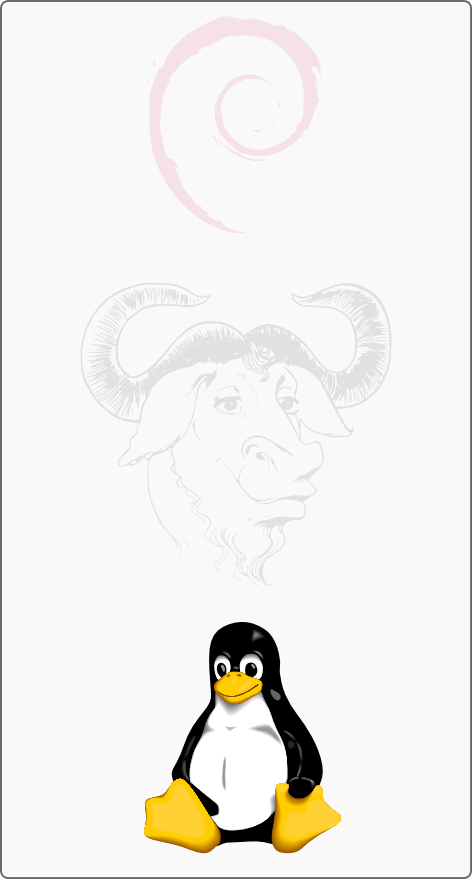
\includegraphics[height=60mm]{../images/debian_gnu_linux_01.png}
    \end{pgfpicture}
    }
\end{frame}

\begin{frame}
\frametitle{GNU}
\begin{block}{}
\begin{itemize}
\item Inițiat de Richard M. Stallman / FSF
\item Este un sistem de operare complet
\item Reprezintă o bază pentru multe alte SO
\item 100\% liber
\item Combinat cu nucleul Linux => GNU/Linux
\end{itemize}
\end{block}
  \raisebox{-15mm}[0pt][0pt]{%
    \begin{pgfpicture}{-48mm}{-36.1mm}{0mm}{0mm}
		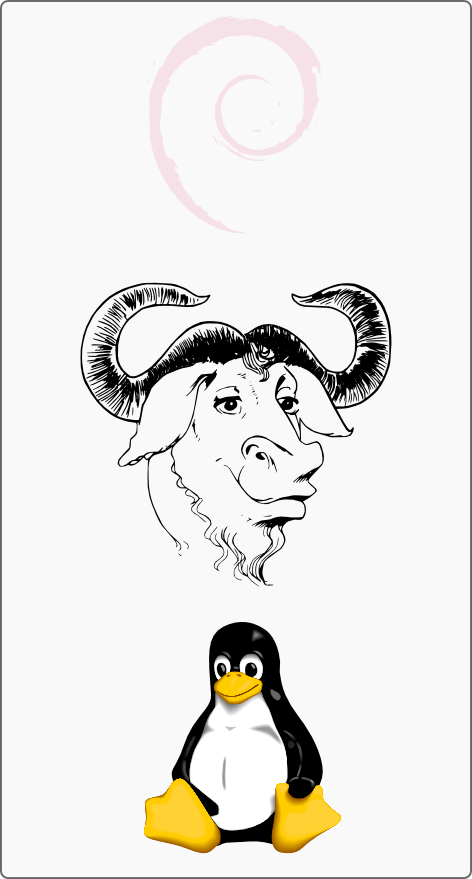
\includegraphics[height=60mm]{../images/debian_gnu_linux_02.png}
    \end{pgfpicture}
    }
\end{frame}

\begin{frame}
\frametitle{Debian}
\begin{block}{}
\begin{itemize}
\item Debian Free Software Guidelines
\item Gestiunea pachetelor: dpkg, apt(itude)
\item Comunitate foarte activă
\item Orientat pe libertate și portabilitate
\item Accesibilitate foarte mare
\end{itemize}
\end{block}
  \raisebox{-15mm}[0pt][0pt]{%
    \begin{pgfpicture}{-48mm}{-35.6mm}{0mm}{0mm}
		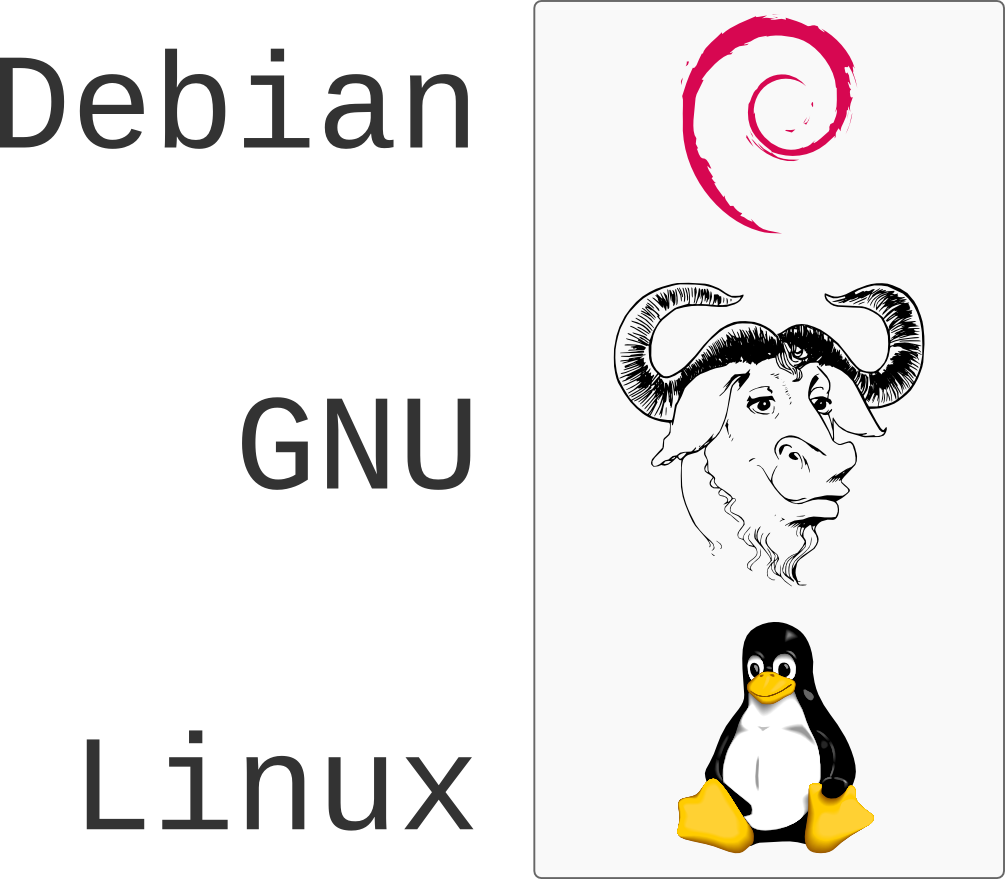
\includegraphics[height=60mm]{../images/debian_gnu_linux_03.png}
    \end{pgfpicture}
    }
\end{frame}

\begin{frame}
\frametitle{DFSG}
\begin{block}
{Indicații extrase din DFSG}
Caracteristici ale unui program liber:\\
\begin{itemize}
\item poate fi redistribuit gratuit
\item include codul sursă
\item permite modificarea / derivarea lui
\item elimină orice discriminare față de persoane / grupuri / intenții
\item asigură păstrarea licenței
\end{itemize}
\end{block}
\begin{normalsize}
\hfill Licențe acceptate ca libere: GPL, BSD, CC-BY-SA
\end{normalsize}
\end{frame}

\begin{frame}
\frametitle{Derivate Debian GNU/Linux}
\begin{block}
{Distribuții construite pe baza Debian}
%
\includegraphics[scale=0.4]{../images/logos/ubuntu_s.png} 
Ubuntu\\
Knoppix\\
Linux Mint Debian Edition (LMDE)\\
Maemo\\
EmDebian\\
siduction\\
Tails
\end{block}
  \raisebox{20mm}[0pt][0pt]{%
    \begin{pgfpicture}{-45mm}{0mm}{0mm}{0mm}
		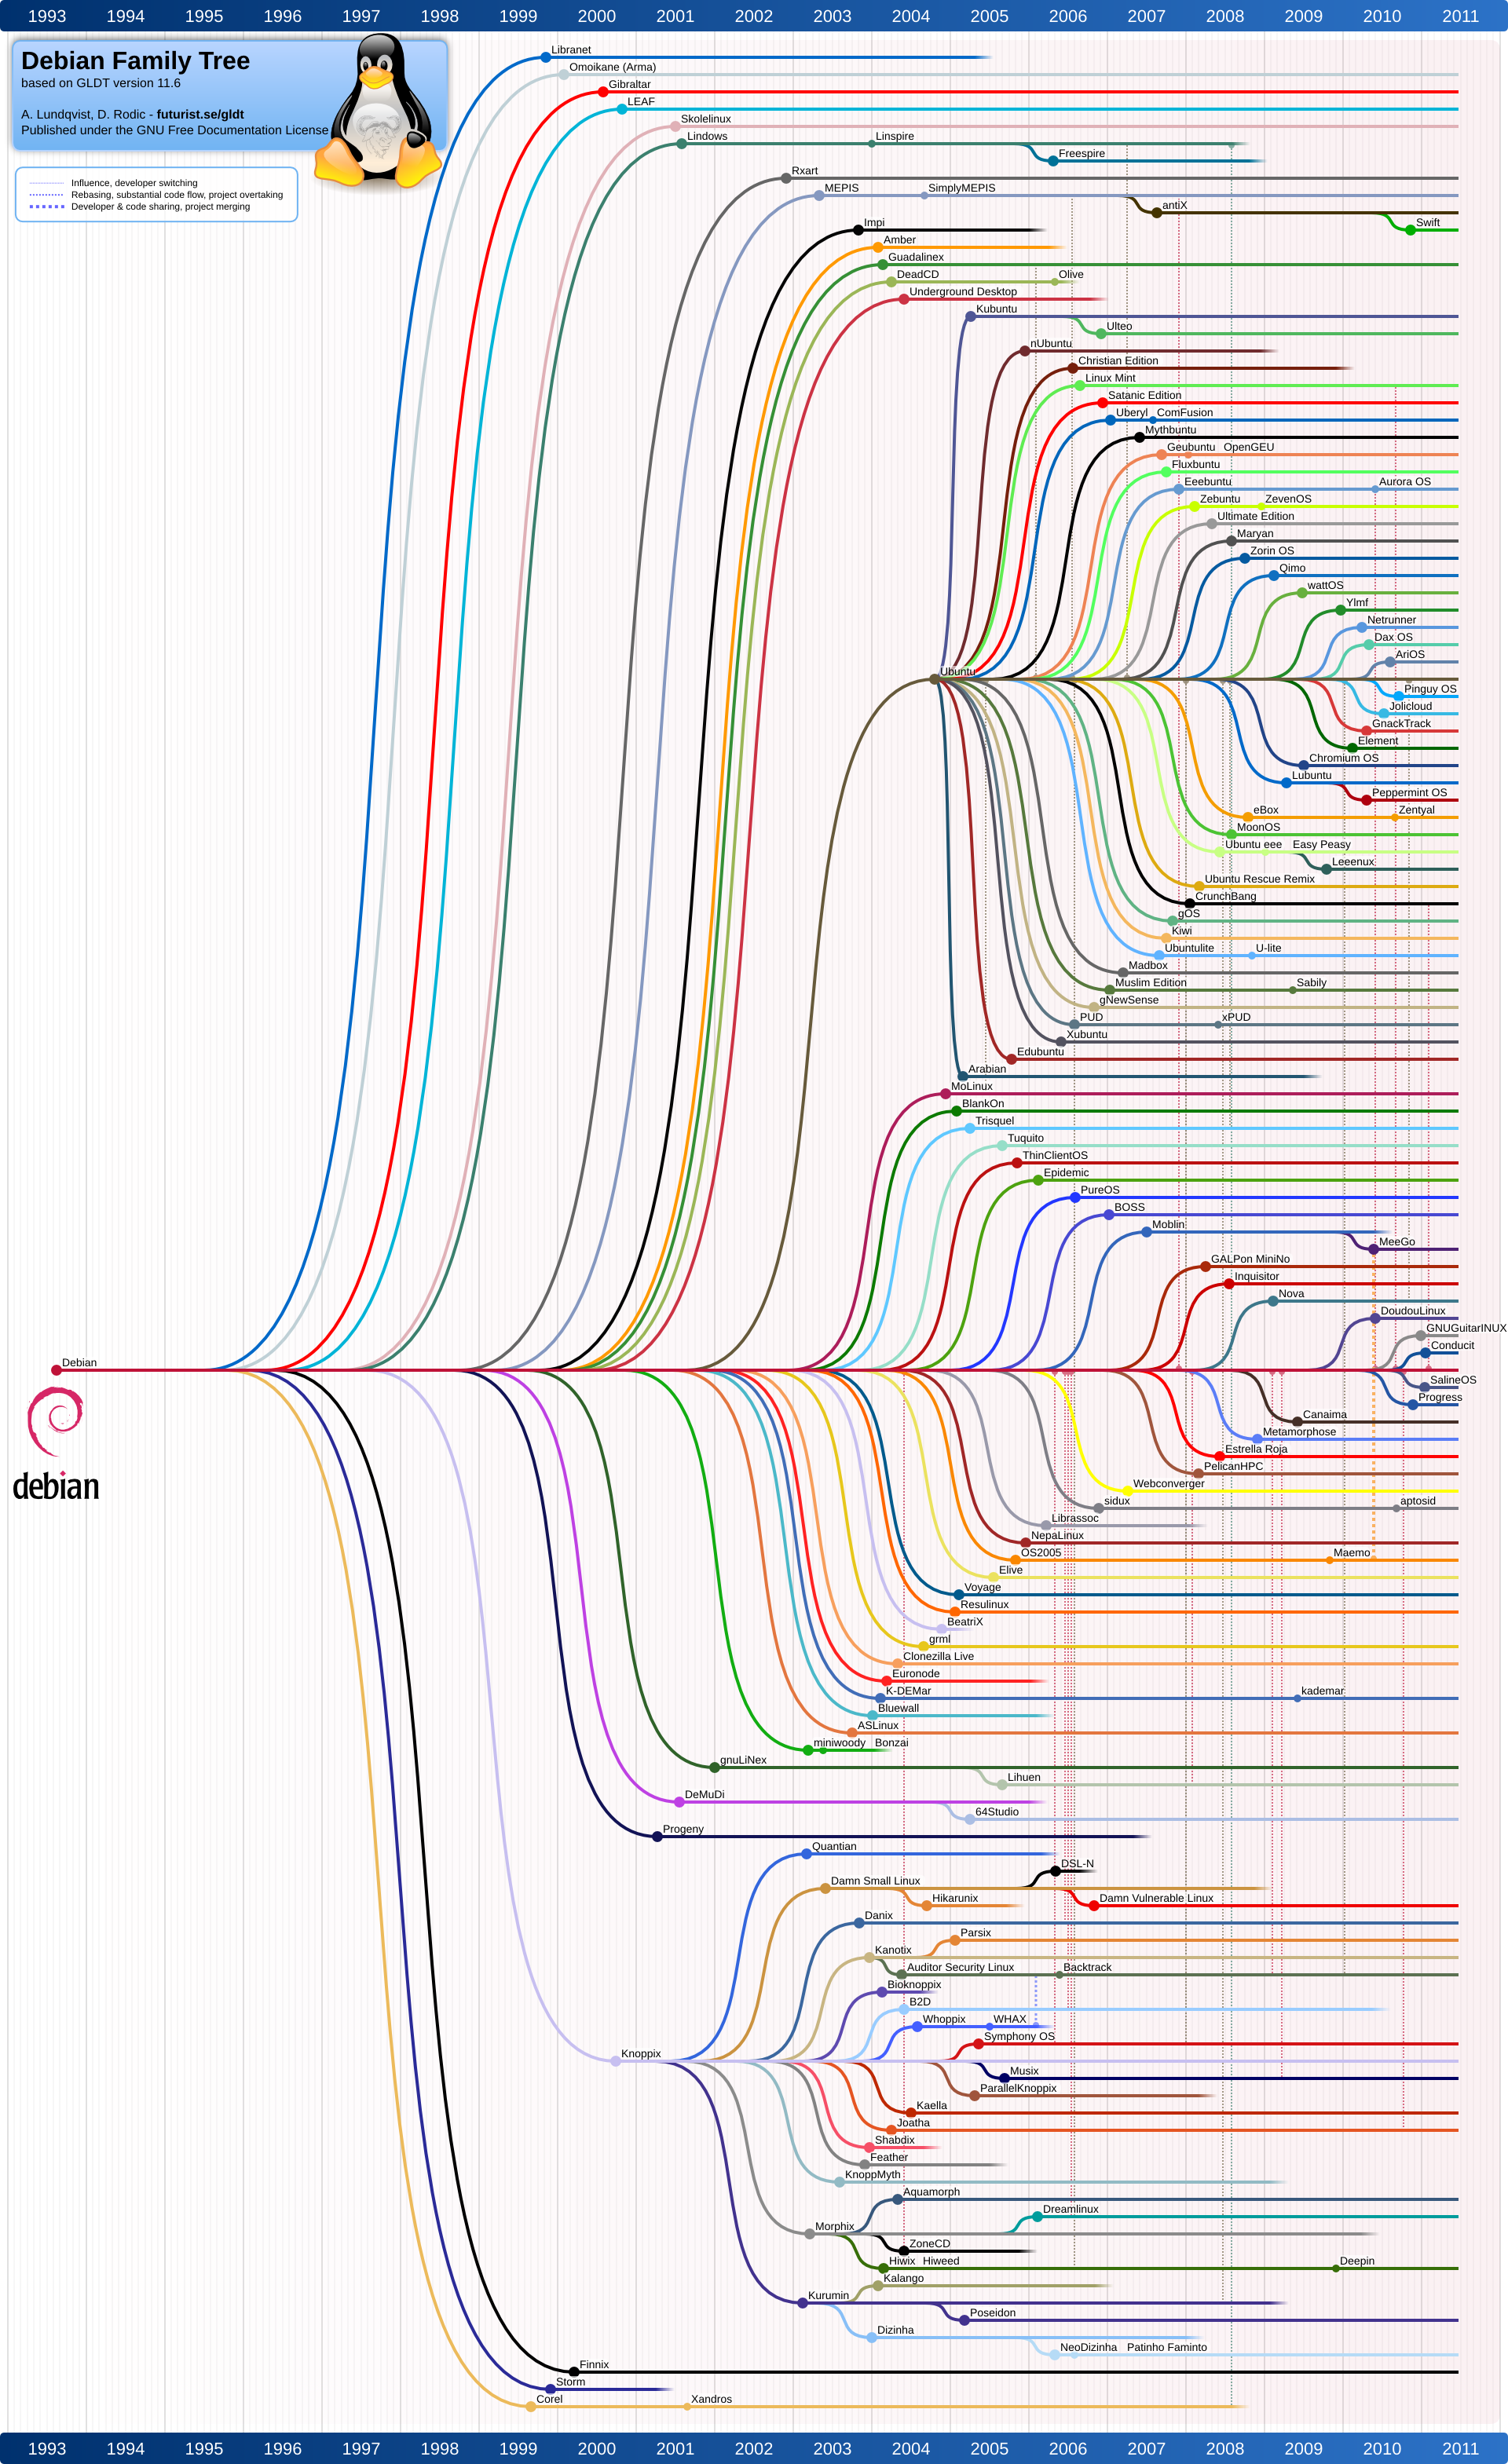
\includegraphics[height=6.5cm]{../images/debian-tree.png}
    \end{pgfpicture}
  }
\end{frame}

%
\subsection{Pure Blends}
\begin{frame}
\frametitle{Variante preconfigurate Debian}
\begin{block}
{Preconfigurate pentru a servi anumitor scopuri specifice}
(en. Debian Pure Blends)\\
\begin{itemize}
\item Debian Junior
	\begin{footnotesize}
		\textcolor{darkred}{(pentru copii între 1 și 99 de ani)}
	\end{footnotesize} 
\item \textcolor{fade}{Debian Med}
	\begin{footnotesize}
		\textcolor{fade}{(practică și cercetare în domeniul medical)}
	\end{footnotesize} 
\item \textcolor{fade}{Skolelinux / Debian Edu}
	\begin{footnotesize}
		\textcolor{fade}{(pentru instituții educaționale)}
	\end{footnotesize} 
\item \textcolor{fade}{Debian Science}
	\begin{footnotesize}
		\textcolor{fade}{(conține programe pentru inginerie și diferite științe)}
	\end{footnotesize} 
\item \textcolor{fade}{DebiChem}
	\begin{footnotesize}
		\textcolor{fade}{(pentru a susține activitatea zilnică a chimiștilor)}
	\end{footnotesize} 
\item \textcolor{fade}{Debian Accessibility}
	\begin{footnotesize}
		\textcolor{fade}{(optimizat pentru utilizatorii cu dizabilități)}
	\end{footnotesize} 
\item \textcolor{fade}{Debian GIS}
	\begin{footnotesize}
		\textcolor{fade}{(util pentru GIS și OpenStreetMap)}
	\end{footnotesize} 
\item \textcolor{fade}{Debian Multimedia}
	\begin{footnotesize}
		\textcolor{fade}{(entuziaști și creatori de conținut multimedia)}
	\end{footnotesize} 
\end{itemize}
\end{block}
\end{frame}

\begin{frame}
\frametitle{Variante preconfigurate Debian}
\begin{block}
{Preconfigurate pentru a servi anumitor scopuri specifice}
(en. Debian Pure Blends)\\
\begin{itemize}
\item Debian Junior
	\begin{footnotesize}
		(pentru copii între 1 și 99 de ani)
	\end{footnotesize} 
\item Debian Med
	\begin{footnotesize}
		\textcolor{darkred}{(practică și cercetare în domeniul medical)}
	\end{footnotesize} 
\item \textcolor{fade}{Skolelinux / Debian Edu}
	\begin{footnotesize}
		\textcolor{fade}{(pentru instituții educaționale)}
	\end{footnotesize} 
\item \textcolor{fade}{Debian Science}
	\begin{footnotesize}
		\textcolor{fade}{(conține programe pentru inginerie și diferite științe)}
	\end{footnotesize} 
\item \textcolor{fade}{DebiChem}
	\begin{footnotesize}
		\textcolor{fade}{(pentru a susține activitatea zilnică a chimiștilor)}
	\end{footnotesize} 
\item \textcolor{fade}{Debian Accessibility}
	\begin{footnotesize}
		\textcolor{fade}{(optimizat pentru utilizatorii cu dizabilități)}
	\end{footnotesize} 
\item \textcolor{fade}{Debian GIS}
	\begin{footnotesize}
		\textcolor{fade}{(util pentru GIS și OpenStreetMap)}
	\end{footnotesize} 
\item \textcolor{fade}{Debian Multimedia}
	\begin{footnotesize}
		\textcolor{fade}{(entuziaști și creatori de conținut multimedia)}
	\end{footnotesize} 
\end{itemize}
\end{block}
\end{frame}

\begin{frame}
\frametitle{Variante preconfigurate Debian}
\begin{block}
{Preconfigurate pentru a servi anumitor scopuri specifice}
(en. Debian Pure Blends)\\
\begin{itemize}
\item Debian Junior
	\begin{footnotesize}
		(pentru copii între 1 și 99 de ani)
	\end{footnotesize} 
\item Debian Med
	\begin{footnotesize}
		(practică și cercetare în domeniul medical)
	\end{footnotesize} 
\item Skolelinux / Debian Edu
	\begin{footnotesize}
		\textcolor{darkred}{(pentru instituții educaționale)}
	\end{footnotesize} 
\item \textcolor{fade}{Debian Science}
	\begin{footnotesize}
		\textcolor{fade}{(conține programe pentru inginerie și diferite științe)}
	\end{footnotesize} 
\item \textcolor{fade}{DebiChem}
	\begin{footnotesize}
		\textcolor{fade}{(pentru a susține activitatea zilnică a chimiștilor)}
	\end{footnotesize} 
\item \textcolor{fade}{Debian Accessibility}
	\begin{footnotesize}
		\textcolor{fade}{(optimizat pentru utilizatorii cu dizabilități)}
	\end{footnotesize} 
\item \textcolor{fade}{Debian GIS}
	\begin{footnotesize}
		\textcolor{fade}{(util pentru GIS și OpenStreetMap)}
	\end{footnotesize} 
\item \textcolor{fade}{Debian Multimedia}
	\begin{footnotesize}
		\textcolor{fade}{(entuziaști și creatori de conținut multimedia)}
	\end{footnotesize} 
\end{itemize}
\end{block}
\end{frame}

\begin{frame}
\frametitle{Variante preconfigurate Debian}
\begin{block}
{Preconfigurate pentru a servi anumitor scopuri specifice}
(en. Debian Pure Blends)\\
\begin{itemize}
\item Debian Junior
	\begin{footnotesize}
		(pentru copii între 1 și 99 de ani)
	\end{footnotesize} 
\item Debian Med
	\begin{footnotesize}
		(practică și cercetare în domeniul medical)
	\end{footnotesize} 
\item Skolelinux / Debian Edu
	\begin{footnotesize}
		(pentru instituții educaționale)
	\end{footnotesize} 
\item Debian Science
	\begin{footnotesize}
		\textcolor{darkred}{(conține programe pentru inginerie și diferite științe)}
	\end{footnotesize} 
\item \textcolor{fade}{DebiChem}
	\begin{footnotesize}
		\textcolor{fade}{(pentru a susține activitatea zilnică a chimiștilor)}
	\end{footnotesize} 
\item \textcolor{fade}{Debian Accessibility}
	\begin{footnotesize}
		\textcolor{fade}{(optimizat pentru utilizatorii cu dizabilități)}
	\end{footnotesize} 
\item \textcolor{fade}{Debian GIS}
	\begin{footnotesize}
		\textcolor{fade}{(util pentru GIS și OpenStreetMap)}
	\end{footnotesize} 
\item \textcolor{fade}{Debian Multimedia}
	\begin{footnotesize}
		\textcolor{fade}{(entuziaști și creatori de conținut multimedia)}
	\end{footnotesize} 
\end{itemize}
\end{block}
\end{frame}

\begin{frame}
\frametitle{Variante preconfigurate Debian}
\begin{block}
{Preconfigurate pentru a servi anumitor scopuri specifice}
(en. Debian Pure Blends)\\
\begin{itemize}
\item Debian Junior
	\begin{footnotesize}
		(pentru copii între 1 și 99 de ani)
	\end{footnotesize} 
\item Debian Med
	\begin{footnotesize}
		(practică și cercetare în domeniul medical)
	\end{footnotesize} 
\item Skolelinux / Debian Edu
	\begin{footnotesize}
		(pentru instituții educaționale)
	\end{footnotesize} 
\item Debian Science
	\begin{footnotesize}
		(conține programe pentru inginerie și diferite științe)
	\end{footnotesize} 
\item DebiChem
	\begin{footnotesize}
		\textcolor{darkred}{(pentru a susține activitatea zilnică a chimiștilor)}
	\end{footnotesize} 
\item \textcolor{fade}{Debian Accessibility}
	\begin{footnotesize}
		\textcolor{fade}{(optimizat pentru utilizatorii cu dizabilități)}
	\end{footnotesize} 
\item \textcolor{fade}{Debian GIS}
	\begin{footnotesize}
		\textcolor{fade}{(util pentru GIS și OpenStreetMap)}
	\end{footnotesize} 
\item \textcolor{fade}{Debian Multimedia}
	\begin{footnotesize}
		\textcolor{fade}{(entuziaști și creatori de conținut multimedia)}
	\end{footnotesize} 
\end{itemize}
\end{block}
\end{frame}

\begin{frame}
\frametitle{Variante preconfigurate Debian}
\begin{block}
{Preconfigurate pentru a servi anumitor scopuri specifice}
(en. Debian Pure Blends)\\
\begin{itemize}
\item Debian Junior
	\begin{footnotesize}
		(pentru copii între 1 și 99 de ani)
	\end{footnotesize} 
\item Debian Med
	\begin{footnotesize}
		(practică și cercetare în domeniul medical)
	\end{footnotesize} 
\item Skolelinux / Debian Edu
	\begin{footnotesize}
		(pentru instituții educaționale)
	\end{footnotesize} 
\item Debian Science
	\begin{footnotesize}
		(conține programe pentru inginerie și diferite științe)
	\end{footnotesize} 
\item DebiChem
	\begin{footnotesize}
		(pentru a susține activitatea zilnică a chimiștilor)
	\end{footnotesize} 
\item Debian Accessibility
	\begin{footnotesize}
		\textcolor{darkred}{(optimizat pentru utilizatorii cu dizabilități)}
	\end{footnotesize} 
\item \textcolor{fade}{Debian GIS}
	\begin{footnotesize}
		\textcolor{fade}{(util pentru GIS și OpenStreetMap)}
	\end{footnotesize} 
\item \textcolor{fade}{Debian Multimedia}
	\begin{footnotesize}
		\textcolor{fade}{(entuziaști și creatori de conținut multimedia)}
	\end{footnotesize} 
\end{itemize}
\end{block}
\end{frame}

\begin{frame}
\frametitle{Variante preconfigurate Debian}
\begin{block}
{Preconfigurate pentru a servi anumitor scopuri specifice}
(en. Debian Pure Blends)\\
\begin{itemize}
\item Debian Junior
	\begin{footnotesize}
		(pentru copii între 1 și 99 de ani)
	\end{footnotesize} 
\item Debian Med
	\begin{footnotesize}
		(practică și cercetare în domeniul medical)
	\end{footnotesize} 
\item Skolelinux / Debian Edu
	\begin{footnotesize}
		(pentru instituții educaționale)
	\end{footnotesize} 
\item Debian Science
	\begin{footnotesize}
		(conține programe pentru inginerie și diferite științe)
	\end{footnotesize} 
\item DebiChem
	\begin{footnotesize}
		(pentru a susține activitatea zilnică a chimiștilor)
	\end{footnotesize} 
\item Debian Accessibility
	\begin{footnotesize}
		(optimizat pentru utilizatorii cu dizabilități)
	\end{footnotesize} 
\item Debian GIS
	\begin{footnotesize}
		\textcolor{darkred}{(util pentru GIS și OpenStreetMap)}
	\end{footnotesize} 
\item \textcolor{fade}{Debian Multimedia}
	\begin{footnotesize}
		\textcolor{fade}{(entuziaști și creatori de conținut multimedia)}
	\end{footnotesize} 
\end{itemize}
\end{block}
\end{frame}

\begin{frame}
\frametitle{Variante preconfigurate Debian}
\begin{block}
{Preconfigurate pentru a servi anumitor scopuri specifice}
(en. Debian Pure Blends)\\
\begin{itemize}
\item Debian Junior
	\begin{footnotesize}
		(pentru copii între 1 și 99 de ani)
	\end{footnotesize} 
\item Debian Med
	\begin{footnotesize}
		(practică și cercetare în domeniul medical)
	\end{footnotesize} 
\item Skolelinux / Debian Edu
	\begin{footnotesize}
		(pentru instituții educaționale)
	\end{footnotesize} 
\item Debian Science
	\begin{footnotesize}
		(conține programe pentru inginerie și diferite științe)
	\end{footnotesize} 
\item DebiChem
	\begin{footnotesize}
		(pentru a susține activitatea zilnică a chimiștilor)
	\end{footnotesize} 
\item Debian Accessibility
	\begin{footnotesize}
		(optimizat pentru utilizatorii cu dizabilități)
	\end{footnotesize} 
\item Debian GIS
	\begin{footnotesize}
		(util pentru GIS și OpenStreetMap)
	\end{footnotesize} 
\item Debian Multimedia
	\begin{footnotesize}
		\textcolor{darkred}{(entuziaști și creatori de conținut multimedia)}
	\end{footnotesize} 
\end{itemize}
\end{block}
\end{frame}

\section{Oriunde, oricând}
\begin{frame}
\frametitle{Debian - oriunde, oricând}
\begin{block}
{Foarte flexibil}
\begin{itemize}
\item are multe forme și dimensiuni
\item poate „locui” în aproape orice condiții
\end{itemize}
\end{block}
\begin{block}
{Mereu aproape}
Grad ridicat de portabilitate => o companie permanentă, „încarnat” în multitudinea de dispozitive din jurul nostru.
\end{block}
\end{frame}

\subsection{Debian e flexibil}
\begin{frame}
\frametitle{Debian poate fi mic...}
\begin{block}
{Embedded}
\begin{itemize}
\item EmDebian
\item Raspbian (Raspberry Pi)
\end{itemize}
\end{block}
\begin{block}
{Tablete}
\begin{itemize}
\item Tabletele Vivaldi vor rula Mer + Plasma Active
\item Debian poate fi instalat pe sisteme cu ecran tactil, la fel ca orice alt sistem
\end{itemize}
\end{block}
\end{frame}

\begin{frame}
\frametitle{...sau impresionant de mare...}
\begin{block}
{Super servere}
\begin{itemize}
\item Proiectul Debian-Beowulf are ca scop eficientizarea instalării de clustere de mari dimensiuni
\item Multe dintre cele mai puternice 500 de supercomputere (conform top500.org) rulează Debian
\end{itemize}
\end{block}
\end{frame}

\begin{frame}[b]
\frametitle{...cam atât de mare:}
  \raisebox{-5mm}[0pt][0pt]{%
    \begin{pgfpicture}{-20mm}{-25mm}{0mm}{0mm}
		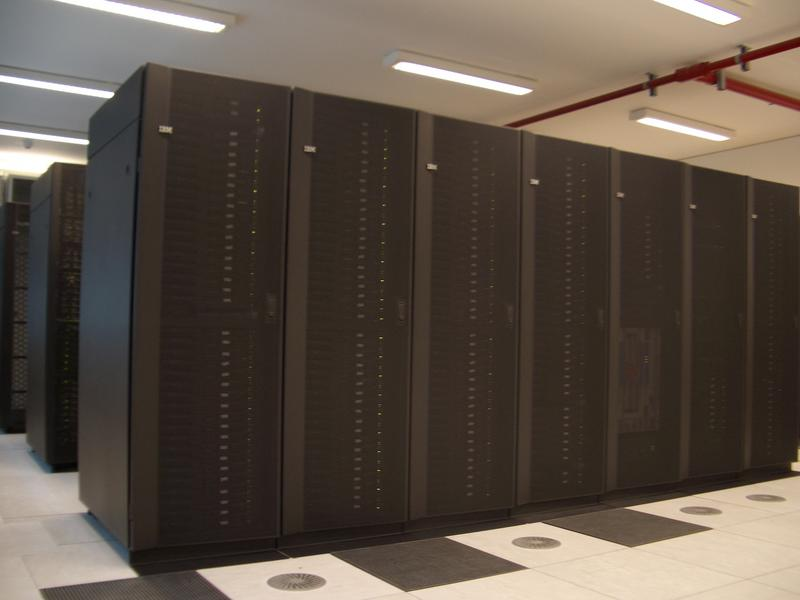
\includegraphics[height=4.5cm]{../images/sc1.jpg}
    \end{pgfpicture}
  }
\begin{block}{}
Clusterul IITAC, University of Dublin, Trinity Centre for High Performance Computing
\end{block}
\end{frame}

\begin{frame}
\frametitle{Domeniul tău e susținut de un sistem Debian?}
  \raisebox{-5mm}[0pt][0pt]{%
    \begin{pgfpicture}{-13mm}{0mm}{0mm}{0mm}
		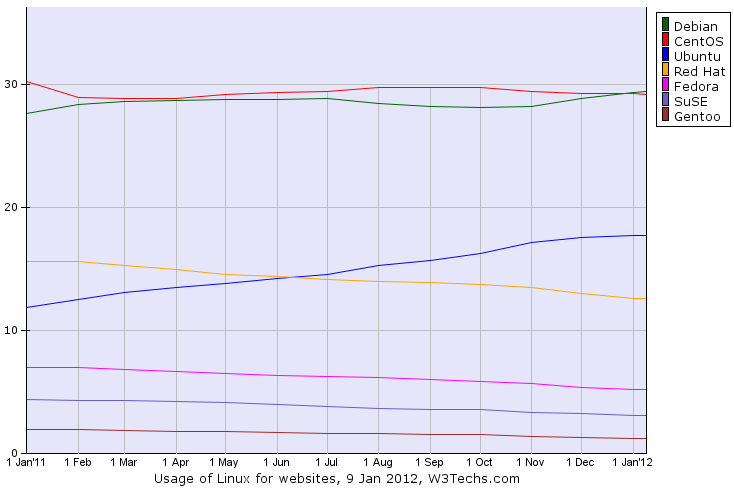
\includegraphics[height=6cm]{../images/debian-server.png}
    \end{pgfpicture}
  }
\end{frame}

\begin{frame}
\frametitle{Embedded + popular}
Se regăsește în dispozitive foarte comune:
  \raisebox{0mm}[0pt][0pt]{%
    \begin{pgfpicture}{-45mm}{-8mm}{0mm}{0mm}
		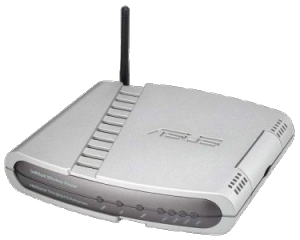
\includegraphics[height=2cm]{../images/asus_wl-500g_deluxe-300x240.png}
    \end{pgfpicture}
    \begin{pgfpicture}{-11mm}{-10mm}{0mm}{0mm}
		
\includegraphics[height=0.2cm]{../images/logos/debwrt.png}
    \end{pgfpicture}
  }
  \raisebox{0mm}[0pt][0pt]{%
    \begin{pgfpicture}{15mm}{3mm}{0mm}{0mm}
		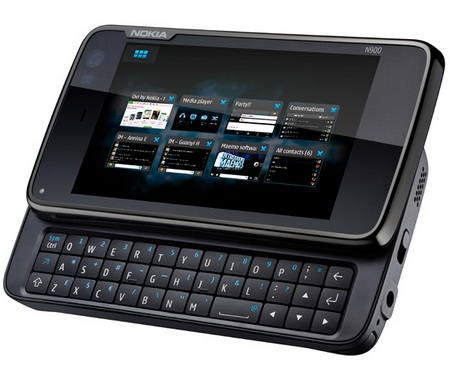
\includegraphics[height=2cm]{../images/n900_maemo.jpg}
    \end{pgfpicture}
    \begin{pgfpicture}{-11mm}{0mm}{0mm}{0mm}
		
\includegraphics[height=0.5cm]{../images/maemo_logo.jpg}
    \end{pgfpicture}
  }
  \raisebox{0mm}[0pt][0pt]{%
    \begin{pgfpicture}{14mm}{12mm}{0mm}{0mm}
		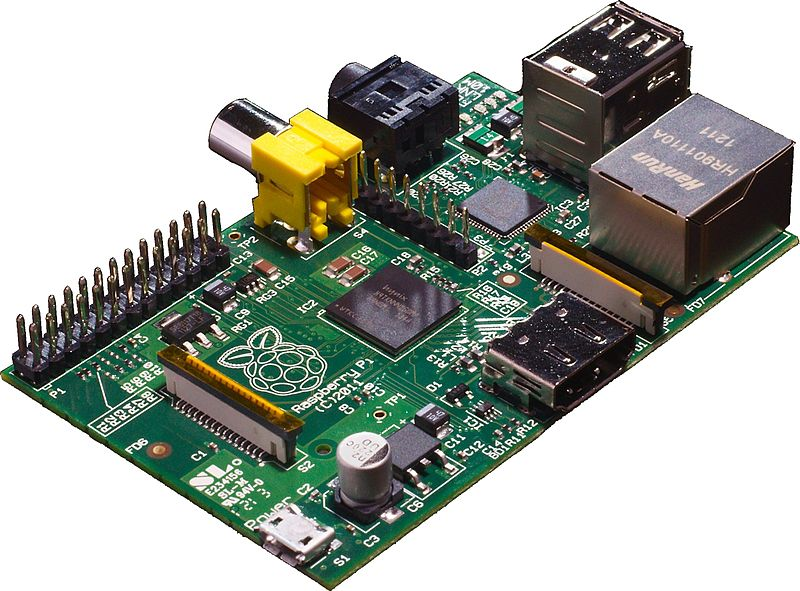
\includegraphics[height=1.6cm]{../images/raspberrypi.jpg}
    \end{pgfpicture}
    \begin{pgfpicture}{-2.5mm}{15mm}{0mm}{0mm}
		
\includegraphics[height=0.5cm]{../images/raspbian_logo.png}
    \end{pgfpicture}
  }
	\begin{itemize}
		\item Routere cu SO derivat din Debian
		\item Nokia au avut mai multe versiuni de\\ 
		sisteme de operare bazate pe Debian
		\item Raspberry Pi => Raspbian
		\item Tablete cu derivate Debian (Mer)
	\end{itemize}
\end{frame}

\begin{frame}
\frametitle{Sisteme desktop și portabile}
	\begin{itemize}
		\item Instalabil pe orice arhitectură desktop sau server\\
		\item Este portat pe mai multe nuclee (Linux, kFreeBSD, HURD)\\
		\item Este tradus în peste 50 de limbi\\
	\end{itemize}
\end{frame}

\subsection{Mereu aproape}
\begin{frame}
\frametitle{Activ 24/7}
\begin{block}
{Dezvoltare pe aproape orice fus orar}
\begin{small}\begin{center}
Datorită distribuției dezvoltatorilor pe glob, Debian este un proiect \color{darkred}permanent activ.\\
\color{darkred}\rule{3cm}{1pt}\\
\color{black}Probleme sau întrebări pot apărea oricând.\\
\color{darkred}\rule{4cm}{1pt}\\
\color{black}De obicei lucrurile (în special software) se strică noaptea sau în weekend.\\
\color{darkred}\rule{4cm}{1pt}\\
\color{black}Este important să poți comunica direct cu creatorii aplicațiilor folosite.
\end{center}
\end{small}
\end{block}
\end{frame}

\begin{frame}
\frametitle{Activ 24/7}
\begin{block}
{Debian nu înseamnă doar dezvoltatori}
\begin{small}
În orice moment, o întreagă armată de administratori de sistem și utilizatori Debian se află online, gata să răspundă oricărei provocări legate de buna funcționare a sistemului.
	\begin{itemize}
		\item IRC: \#debian pe \color{darkred}irc.debian.net\\
		\item \color{black}Liste de discuții: \color{darkred}lists.debian.org\\
		\item \color{black}Forumuri: \color{darkred}forums.debian.net \color{black}sau \color{darkred}forum.debian.org.ro\\
	\end{itemize}
\end{small}
\end{block}
\end{frame}

\begin{frame}
\frametitle{Harta dezvoltatorilor Debian}
  \raisebox{0mm}[0pt][0pt]{%
    \begin{pgfpicture}{-7.5mm}{5mm}{0mm}{0mm}
		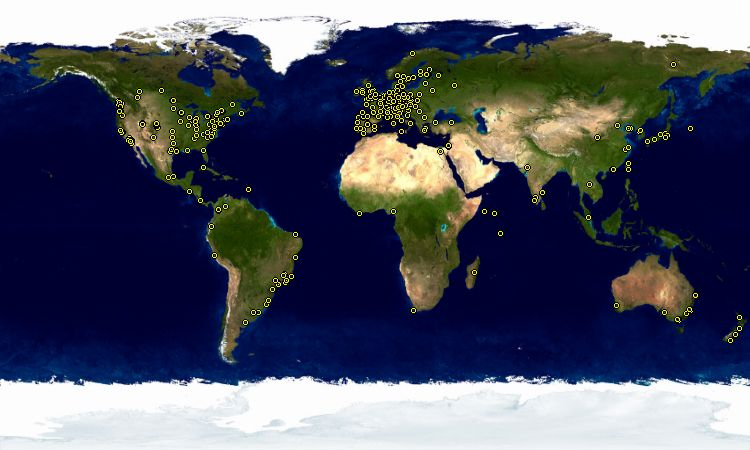
\includegraphics[height=6.5cm]{../images/developers.map.jpeg}
    \end{pgfpicture}
  }
\end{frame}

\section{Avantaje}
\begin{frame}
\frametitle{Generalități}
\begin{block}
{Avantajele utilizării Debian GNU/Linux}
\begin{itemize}
	\item Comunitatea este mare, activă și prietenoasă
	\item Proiectul este matur, stabil și previzibil
	\item Apreciem transparența, atât cea decizională, cât și în implementările efectuate
\end{itemize}
\end{block}
\end{frame}

\begin{frame}
\frametitle{Cuvântul cheie - diversitate}
\begin{block}
{Oricine poate folosi Debian GNU/Linux}
Fiecare poate găsi o combinație unică și productivă în utilizarea sistemului de operare.\\
În sprijinul acestei idei au apărut „Pure Blends”, demonstrând eficiența într-o varietate foarte mare de cerințe practice.
\begin{itemize}
	\item Elevi si studenți din orice domeniu
	\item Cercetători și oameni de știință
	\item Entuziaști ai tehnologiei
\end{itemize}
\end{block}
\end{frame}

\subsection{Utilizatori}
\begin{frame}
\frametitle{Stabilitate și maturitate}
\begin{block}
{Avantajele utilizării Debian GNU/Linux}
\begin{itemize}
	\item Cu toții vrem un sistem stabil...
	\item rapid...
	\item previzibil...
	\item sigur.
\end{itemize}
În plus, securitatea sistemului este limitată doar de intențiile și priceperea utilizatorilor acestuia.
\end{block}
\end{frame}

\begin{frame}
\frametitle{Extrem de personalizabil}
\begin{block}
{Ai propria viziune despre mediul de lucru?}
Dacă da, vei fi plăcut impresionat. În lumea sistemelor GNU/Linux, a avea o multitudine de variante este ceva extrem de comun.
\end{block}
\begin{block}
{Îți place să experimentezi?}
Nu există teren mai solid și mai diversificat. Alege să-ți creezi propria experiență unică, combinând piese din puzzle-ul programelor libere!
\end{block}
\end{frame}

\subsection{Dezvoltatori}
\begin{frame}
\frametitle{Facilitarea procesului de creație}
\begin{block}
{Sistemul de operare este un aliat, nu un sabotor}
\begin{itemize}
	\item O multitudine de instrumente
	\item Posibilitate de dezvoltare pentru mai multe platforme
	\item Integrare solidă cu sistemul de operare
\end{itemize}
\end{block}
\end{frame}

\begin{frame}
\frametitle{Acces la structura internă a sistemului}
\begin{block}
{...sau cum să învățăm din codul sursă}
\begin{itemize}
	\item Putem studia și modifica orice element al sistemului
	\item Studierea codului deja scris facilitează de multe ori producerea de cod superior
	\item Ne putem ajusta sistemul de operare propriilor tehnici de dezvoltare
\end{itemize}
\end{block}
\end{frame}

\section{Comunitatea Debian}
\begin{frame}
\frametitle{Comunitatea Debian}
\begin{block}
{Ce are special?}
\begin{itemize}
\item Membri din domenii diferite, implicați într-un proiect comun
\item Debian nu are (în mare parte) termene limită; se lucrează cu plăcere și din plăcere!
\item Deciziile sunt luate de comun acord între dezvoltatori (și utilizatori, unde este aplicabil)
\end{itemize}
  \raisebox{0mm}[0mm][0pt]{%
    \begin{pgfpicture}{-50mm}{10mm}{0mm}{0mm}
		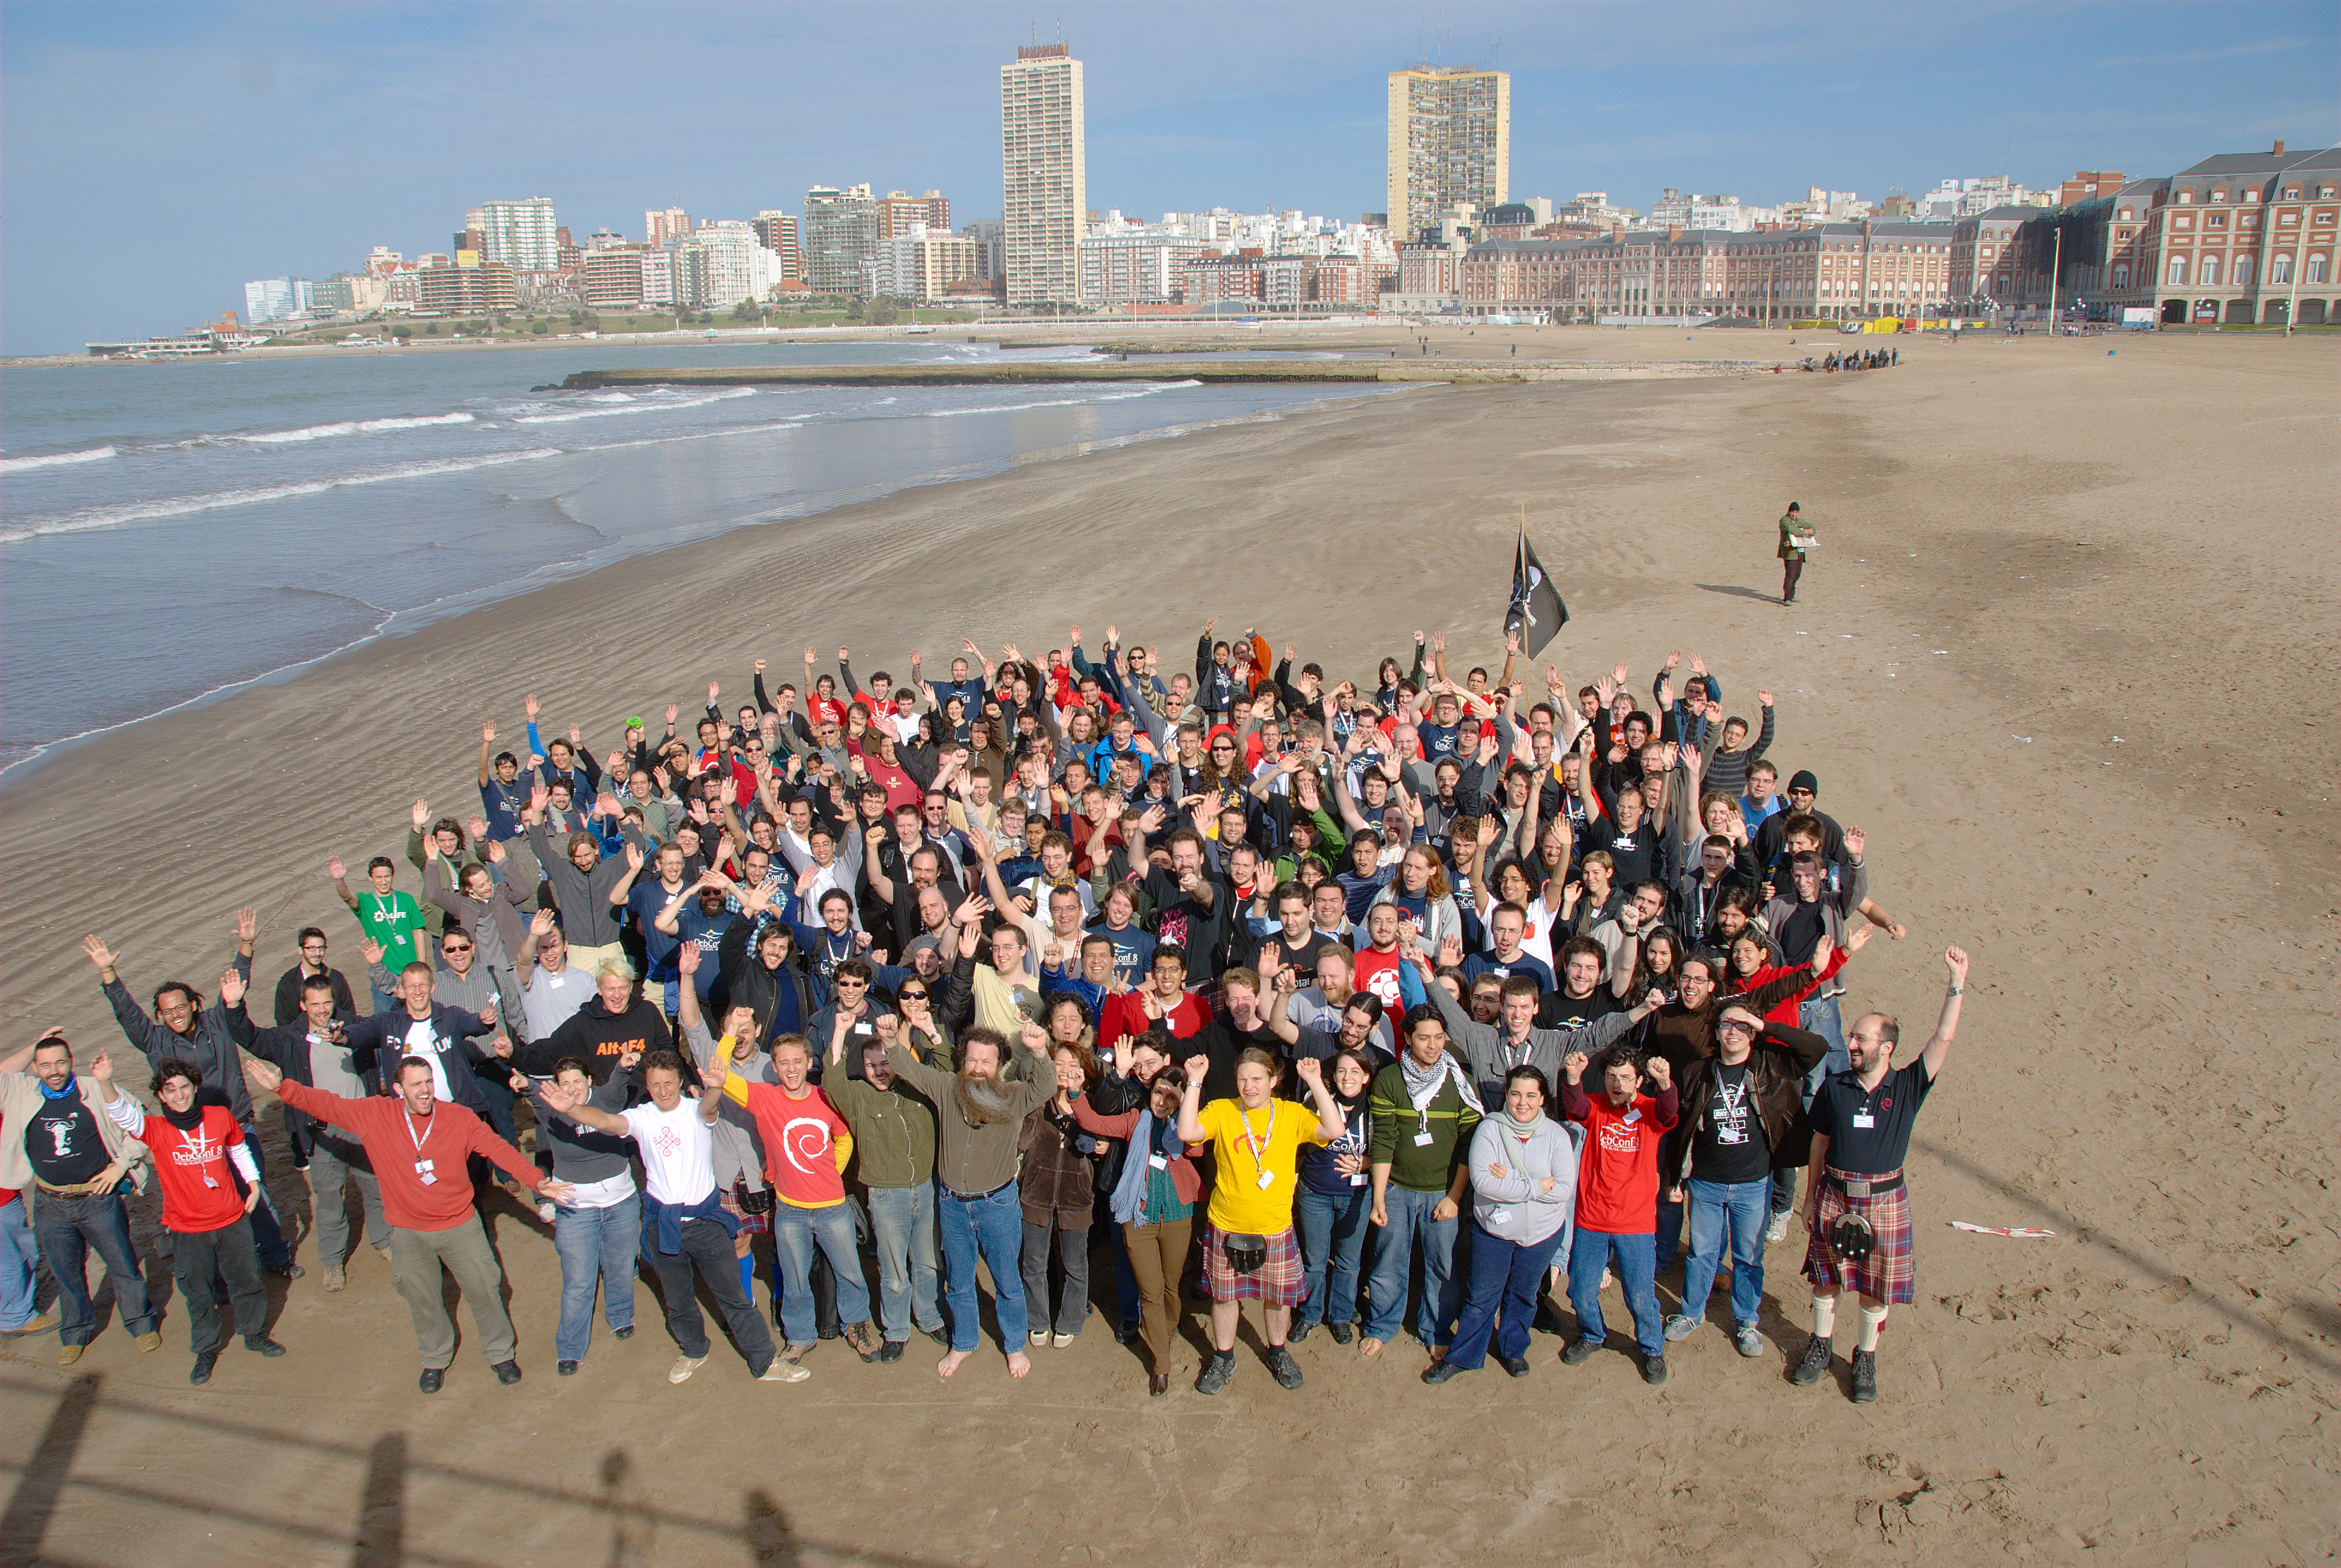
\includegraphics[height=2cm]{../images/debconf12.jpg}
    \end{pgfpicture}
  }
\end{block}
\end{frame}

\subsection{Implicare?}
\begin{frame}
\frametitle{}
\begin{small}
Concept cheie: „do-ocracy” - dacă ai idei, ești liber să le încerci.
\end{small}
\begin{block}
{Părțile bune}
\begin{itemize}
\item Poți influența direct cursul proiectului
\item Ocazia de a lucra cu adevărați profesioniști
\item Indiferent ce știi să faci / cât timp ai, poți fi productiv
\item Recunoașterea imediată și obiectivă a realizărilor
\end{itemize}
\end{block}
\begin{block}
{Părțile rele}
\begin{itemize}
\item Deciziile (bune) se iau greu
\item Responsabilitatea crește cu numărul distribuțiilor derivate
\item Dispersarea pe glob face sincronizările online foarte dificile
\end{itemize}
\end{block}
\end{frame}

\begin{frame}
\frametitle{Implicare: Traduceri (1/5)}
\begin{block}{}
Traducerile sunt cea mai simplă cale de a participa la dezvoltarea Debian:\\
\begin{itemize}
\item Documentație
\item Pagini web (debian.org / wiki.debian.org)
\item Manuale
\item Articole din presa scrisă și online
\item Debian Project News (\textbf{DPN})
\end{itemize}
\end{block}
\end{frame}

\begin{frame}
\frametitle{Implicare: Identificarea și raportarea erorilor (2/5)}
\begin{block}{}
Debian Bug Tracking System\\
\begin{itemize}
\item Trierea / validarea rapoartelor deschise
\item Completarea descrierilor
\item Raportarea de noi erori
\item Solicitarea de noi funcționalități
\item Corelarea și marcarea corespunzătoare a rapoartelor existente
\end{itemize}
\end{block}
\end{frame}

\begin{frame}
\frametitle{Implicare: Pregătirea de pachete (3/5)}
\begin{block}{}
Fiecare program are nevoie de un pachet compatibil cu SO\\
\begin{itemize}
\item Se respectă regulile specifice managerului de pachete
\item Autorul original al programului trebuie consultat periodic pentru a păstra pachetele actualizate (reîmpachetarea noilor versiuni)
\item Deseori este nevoie să fie preluate pachetele altui administrator
\item Se urmărește tranziția acestuia în cadrul procesului de dezvoltare
\item Erorile raportate trebuiesc triate, eventual trimise către autorul original (en. upstream)
\end{itemize}
\end{block}
\end{frame}

\begin{frame}
\frametitle{Implicare: Contribuirea cu cod (4/5)}
\begin{block}{}
Repararea erorilor raportate\\
\begin{itemize}
\item Debian Bug Tracking System (bugs.debian.org)
\item Verificare
\item Reparare
\item Trimiterea soluției către administratorii pachetului
\end{itemize}
\end{block}
\begin{block}{}
Scrierea de cod nou\\
\begin{itemize}
\item De obicei realizată de dezvoltatorii cu experiență în cadrul proiectului
\end{itemize}
\end{block}
\end{frame}

\begin{frame}
\frametitle{Implicare: Proiectarea de noi machete grafice (5/5)}
\begin{block}{}
Interfața unui mediu de lucru e un aspect important?\\
Dacă da, ai viziunea și aptitudinile necesare?
\begin{itemize}
\item Poți contribui la grafica Debian, fără a fi necesară o implicare anterioară în cadrul proiectului
\item Înainte de fiecare versiune, tema grafică este aleasă de comun acord utilizatori / dezvoltatori
\item Există și alte moduri de completare a graficii: seturi, palete de culori, teme pentru web, materiale promoționale etc.
\end{itemize}
\end{block}
\end{frame}

\subsection{Comunitatea din România}
\begin{frame}
\frametitle{Proiecte și planuri}
\begin{block}{Ce urmează?}
\begin{itemize}
\item Traducerea documentației existente
\item Organizarea a cât mai multe evenimente
\item Contribuirea cu cod către Debian GNU/Linux
\end{itemize}
\end{block}
\begin{block}{Ce vrem să obținem?}
\begin{itemize}
\item Un număr crescut de contribuții 100\% românești
\item Mai mulți membri și dezvoltatori în cadrul Debian
\end{itemize}
\end{block}
\end{frame}

\section{Final} 
\begin{frame}
\centerline{Întrebări?}
\end{frame}
% End of slides
\end{document} 
